\documentclass[conference,compsoc]{IEEEtran}
 
\usepackage{datetime}
\usepackage{xcolor}
\usepackage[colorlinks=true]{hyperref}
\usepackage{glossaries}
\usepackage{varioref}

\let\labelindent\relax
\usepackage[inline,shortlabels]{enumitem}

\newcounter{tdel}
\newcounter{sdel}

\newcommand{\AC}[1]{\noindent{\color{orange}{{\bf[AC:}{{#1}}}]}}
\newcommand{\KB}[1]{\noindent{\color{purple}{{\bf[KB:}{{#1}}}]}}

\glsdisablehyper
\newacronym{bsp}{BSP}{Bachelor Semester Project}
\newacronym{e4l}{E4L}{Energy4Life}
\newacronym{ms}{MS}{Microservice}
\newacronym{cicd}{CI/CD}{Continuous Integration and Continuous Deployment}

% *** CITATION PACKAGES ***
%
\ifCLASSOPTIONcompsoc
  % IEEE Computer Society needs nocompress option
  % requires cite.sty v4.0 or later (November 2003)
  \usepackage[nocompress]{cite}
\else
  % normal IEEE
  \usepackage{cite}
\fi
% cite.sty was written by Donald Arseneau
% V1.6 and later of IEEEtran pre-defines the format of the cite.sty package
% \cite{} output to follow that of the IEEE. Loading the cite package will
% result in citation numbers being automatically sorted and properly
% "compressed/ranged". e.g., [1], [9], [2], [7], [5], [6] without using
% cite.sty will become [1], [2], [5]--[7], [9] using cite.sty. cite.sty's
% \cite will automatically add leading space, if needed. Use cite.sty's
% noadjust option (cite.sty V3.8 and later) if you want to turn this off
% such as if a citation ever needs to be enclosed in parenthesis.
% cite.sty is already installed on most LaTeX systems. Be sure and use
% version 5.0 (2009-03-20) and later if using hyperref.sty.
% The latest version can be obtained at:
% http://www.ctan.org/pkg/cite
% The documentation is contained in the cite.sty file itself.
%
% Note that some packages require special options to format as the Computer
% Society requires. In particular, Computer Society  papers do not use
% compressed citation ranges as is done in typical IEEE papers
% (e.g., [1]-[4]). Instead, they list every citation separately in order
% (e.g., [1], [2], [3], [4]). To get the latter we need to load the cite
% package with the nocompress option which is supported by cite.sty v4.0
% and later.

% *** GRAPHICS RELATED PACKAGES ***
%
\ifCLASSINFOpdf
	\usepackage[pdftex]{graphicx}
  % declare the path(s) where your graphic files are
  % \graphicspath{{../pdf/}{../jpeg/}}
  % and their extensions so you won't have to specify these with
  % every instance of \includegraphics
  % \DeclareGraphicsExtensions{.pdf,.jpeg,.png}
\else
  % or other class option (dvipsone, dvipdf, if not using dvips). graphicx
  % will default to the driver specified in the system graphics.cfg if no
  % driver is specified.
  % \usepackage[dvips]{graphicx}
  % declare the path(s) where your graphic files are
  % \graphicspath{{../eps/}}
  % and their extensions so you won't have to specify these with
  % every instance of \includegraphics
  % \DeclareGraphicsExtensions{.eps}
\fi
% graphicx was written by David Carlisle and Sebastian Rahtz. It is
% required if you want graphics, photos, etc. graphicx.sty is already
% installed on most LaTeX systems. The latest version and documentation
% can be obtained at: 
% http://www.ctan.org/pkg/graphicx
% Another good source of documentation is "Using Imported Graphics in
% LaTeX2e" by Keith Reckdahl which can be found at:
% http://www.ctan.org/pkg/epslatex
%
% latex, and pdflatex in dvi mode, support graphics in encapsulated
% postscript (.eps) format. pdflatex in pdf mode supports graphics
% in .pdf, .jpeg, .png and .mps (metapost) formats. Users should ensure
% that all non-photo figures use a vector format (.eps, .pdf, .mps) and
% not a bitmapped formats (.jpeg, .png). The IEEE frowns on bitmapped formats
% which can result in "jaggedy"/blurry rendering of lines and letters as
% well as large increases in file sizes.
%
% You can find documentation about the pdfTeX application at:
% http://www.tug.org/applications/pdftex


% *** MATH PACKAGES ***
%
%\usepackage{amsmath}
% A popular package from the American Mathematical Society that provides
% many useful and powerful commands for dealing with mathematics.
%
% Note that the amsmath package sets \interdisplaylinepenalty to 10000
% thus preventing page breaks from occurring within multiline equations. Use:
%\interdisplaylinepenalty=2500
% after loading amsmath to restore such page breaks as IEEEtran.cls normally
% does. amsmath.sty is already installed on most LaTeX systems. The latest
% version and documentation can be obtained at:
% http://www.ctan.org/pkg/amsmath

% *** SPECIALIZED LIST PACKAGES ***
%
%\usepackage{algorithmic}
% algorithmic.sty was written by Peter Williams and Rogerio Brito.
% This package provides an algorithmic environment fo describing algorithms.
% You can use the algorithmic environment in-text or within a figure
% environment to provide for a floating algorithm. Do NOT use the algorithm
% floating environment provided by algorithm.sty (by the same authors) or
% algorithm2e.sty (by Christophe Fiorio) as the IEEE does not use dedicated
% algorithm float types and packages that provide these will not provide
% correct IEEE style captions. The latest version and documentation of
% algorithmic.sty can be obtained at:
% http://www.ctan.org/pkg/algorithms
% Also of interest may be the (relatively newer and more customizable)
% algorithmicx.sty package by Szasz Janos:
% http://www.ctan.org/pkg/algorithmicx


% *** ALIGNMENT PACKAGES ***
%
%\usepackage{array}
% Frank Mittelbach's and David Carlisle's array.sty patches and improves
% the standard LaTeX2e array and tabular environments to provide better
% appearance and additional user controls. As the default LaTeX2e table
% generation code is lacking to the point of almost being broken with
% respect to the quality of the end results, all users are strongly
% advised to use an enhanced (at the very least that provided by array.sty)
% set of table tools. array.sty is already installed on most systems. The
% latest version and documentation can be obtained at:
% http://www.ctan.org/pkg/array

% IEEEtran contains the IEEEeqnarray family of commands that can be used to
% generate multiline equations as well as matrices, tables, etc., of high
% quality.

% *** SUBFIGURE PACKAGES ***
%\ifCLASSOPTIONcompsoc
%  \usepackage[caption=false,font=footnotesize,labelfont=sf,textfont=sf]{subfig}
%\else
%  \usepackage[caption=false,font=footnotesize]{subfig}
%\fi
% subfig.sty, written by Steven Douglas Cochran, is the modern replacement
% for subfigure.sty, the latter of which is no longer maintained and is
% incompatible with some LaTeX packages including fixltx2e. However,
% subfig.sty requires and automatically loads Axel Sommerfeldt's caption.sty
% which will override IEEEtran.cls' handling of captions and this will result
% in non-IEEE style figure/table captions. To prevent this problem, be sure
% and invoke subfig.sty's "caption=false" package option (available since
% subfig.sty version 1.3, 2005/06/28) as this is will preserve IEEEtran.cls
% handling of captions.
% Note that the Computer Society format requires a sans serif font rather
% than the serif font used in traditional IEEE formatting and thus the need
% to invoke different subfig.sty package options depending on whether
% compsoc mode has been enabled.
%
% The latest version and documentation of subfig.sty can be obtained at:
% http://www.ctan.org/pkg/subfig

% *** FLOAT PACKAGES ***
%
%\usepackage{fixltx2e}
% fixltx2e, the successor to the earlier fix2col.sty, was written by
% Frank Mittelbach and David Carlisle. This package corrects a few problems
% in the LaTeX2e kernel, the most notable of which is that in current
% LaTeX2e releases, the ordering of single and double column floats is not
% guaranteed to be preserved. Thus, an unpatched LaTeX2e can allow a
% single column figure to be placed prior to an earlier double column
% figure.
% Be aware that LaTeX2e kernels dated 2015 and later have fixltx2e.sty's
% corrections already built into the system in which case a warning will
% be issued if an attempt is made to load fixltx2e.sty as it is no longer
% needed.
% The latest version and documentation can be found at:
% http://www.ctan.org/pkg/fixltx2e

%\usepackage{stfloats}
% stfloats.sty was written by Sigitas Tolusis. This package gives LaTeX2e
% the ability to do double column floats at the bottom of the page as well
% as the top. (e.g., "\begin{figure*}[!b]" is not normally possible in
% LaTeX2e). It also provides a command:
%\fnbelowfloat
% to enable the placement of footnotes below bottom floats (the standard
% LaTeX2e kernel puts them above bottom floats). This is an invasive package
% which rewrites many portions of the LaTeX2e float routines. It may not work
% with other packages that modify the LaTeX2e float routines. The latest
% version and documentation can be obtained at:
% http://www.ctan.org/pkg/stfloats
% Do not use the stfloats baselinefloat ability as the IEEE does not allow
% \baselineskip to stretch. Authors submitting work to the IEEE should note
% that the IEEE rarely uses double column equations and that authors should try
% to avoid such use. Do not be tempted to use the cuted.sty or midfloat.sty
% packages (also by Sigitas Tolusis) as the IEEE does not format its papers in
% such ways.
% Do not attempt to use stfloats with fixltx2e as they are incompatible.
% Instead, use Morten Hogholm'a dblfloatfix which combines the features
% of both fixltx2e and stfloats:
%
% \usepackage{dblfloatfix}
% The latest version can be found at:
% http://www.ctan.org/pkg/dblfloatfix

% *** PDF, URL AND HYPERLINK PACKAGES ***
%
%\usepackage{url}
% url.sty was written by Donald Arseneau. It provides better support for
% handling and breaking URLs. url.sty is already installed on most LaTeX
% systems. The latest version and documentation can be obtained at:
% http://www.ctan.org/pkg/url
% Basically, \url{my_url_here}.

% *** Do not adjust lengths that control margins, column widths, etc. ***
% *** Do not use packages that alter fonts (such as pslatex).         ***
% There should be no need to do such things with IEEEtran.cls V1.6 and later.
% (Unless specifically asked to do so by the journal or conference you plan
% to submit to, of course. )

% correct bad hyphenation here
\hyphenation{op-tical net-works semi-conduc-tor}
   
\usepackage{hyperref}
 
\begin{document}
% 
% paper title
% Titles are generally capitalized except for words such as a, an, and, as,
% at, but, by, for, in, nor, of, on, or, the, to and up, which are usually
% not capitalized unless they are the first or last word of the title.
% Linebreaks \\ can be used within to get better formatting as desired.
% Do not put math or special symbols in the title.
\title{Microservices Architecture on Energy4Life Monolithic Application\\
{\small \today~-~\currenttime}}

 
% author names and affiliations
% use a multiple column layout for up to three different
% affiliations
\author{\IEEEauthorblockN{Kevin L.\ Biewesch}
\IEEEauthorblockA{University of Luxembourg\\
Email: kevin.biewesch.001@student.uni.lu}
\and 
\IEEEauthorblockN{Alfredo Capozucca}
\IEEEauthorblockA{University of Luxembourg\\
Email: alfredo.capozucca@uni.lu}%
}

% conference papers do not typically use \thanks and this command
% is locked out in conference mode. If really needed, such as for
% the acknowledgment of grants, issue a \IEEEoverridecommandlockouts
% after \documentclass

% for over three affiliations, or if they all won't fit within the width
% of the page (and note that there is less available width in this regard for
% compsoc conferences compared to traditional conferences), use this
% alternative format:
% 
%\author{\IEEEauthorblockN{Michael Shell\IEEEauthorrefmark{1},
%Homer Simpson\IEEEauthorrefmark{2},
%James Kirk\IEEEauthorrefmark{3}, 
%Montgomery Scott\IEEEauthorrefmark{3} and
%Eldon Tyrell\IEEEauthorrefmark{4}}
%\IEEEauthorblockA{\IEEEauthorrefmark{1}School of Electrical and Computer Engineering\\
%Georgia Institute of Technology,
%Atlanta, Georgia 30332--0250\\ Email: see http://www.michaelshell.org/contact.html}
%\IEEEauthorblockA{\IEEEauthorrefmark{2}Twentieth Century Fox, Springfield, USA\\
%Email: homer@thesimpsons.com}
%\IEEEauthorblockA{\IEEEauthorrefmark{3}Starfleet Academy, San Francisco, California 96678-2391\\
%Telephone: (800) 555--1212, Fax: (888) 555--1212}
%\IEEEauthorblockA{\IEEEauthorrefmark{4}Tyrell Inc., 123 Replicant Street, Los Angeles, California 90210--4321}}




% use for special paper notices
%\IEEEspecialpapernotice{(Invited Paper)}




% make the title area
\maketitle

% As a general rule, do not put math, special symbols or citations
% in the abstract
\begin{abstract}
	% {\color{gray}
% This document is a template for the scientific and technical (S\&T for short) report that is to be delivered by any BiCS student at the end of each Bachelor Semester Project (BSP). The Latex source files are available at:\\
% \href{https://github.com/nicolasguelfi/lu.uni.course.bics.global}{{\underline{\textbf{https://github.com/nicolasguelfi/lu.uni.course.bics.global}}}}\\
  
% This template is to be used using the Latex document preparation system or using any document preparation system. The whole document should be in between 6000 to 8000 words~\footnote{i.e. approximately 12 to 16 pages double columns} (excluding the annexes) and the proportions must be preserved. The other documents to be delivered (summaries, \ldots) should have their format adapted from this template.
% }

In the domain of software engineering, microservices are an emanate
approach for building applications. Its benefits are numerous and
target the long-term development of a product---most notably
\emph{scalability} to meet growing needs and \emph{maintenance} over the whole
life-cycle.

During this project we inspected what a microservice is and how DevOps
plays a key role in this new architectural style, the insights of
which are presented in this report.

The \emph{Energy4Life} monolithic application served as our use case
for creating a microservice. The latter is an independent
service---meaning that it should be deployable independently from
Energy4Life or any other service---that displays data from the former.
Our intention was for it to portray a proof of concept\footnote{If
needed, our microservice may be extended or re-purposed to be more
useful to the Energy4Life ecosystem.} showing that you can indeed deploy an
microservice adjacent to a monolith.  We will present the whole
process of creating this service along with the problems we faced and
how we circumvented them.

\end{abstract}

% no keywords

% For peer review papers, you can put extra information on the cover
% page as needed:
% \ifCLASSOPTIONpeerreview
% \begin{center} \bfseries EDICS Category: 3-BBND \end{center}
% \fi
%
% For peerreview papers, this IEEEtran command inserts a page break and
% creates the second title. It will be ignored for other modes.
\IEEEpeerreviewmaketitle

% no \IEEEPARstart
\section{Introduction (± 5\% of total words)}

Traditionally, when developing software the most common way to
approach it is by making a monolithic application.
\cite{ms-challenges} This entails that the developer teams are split
vertically \cite{ms-challenges} according to application layers
\cite{ms-definition}---for instance one party will be responsible
solely for the database, yet another will take care of the actual
server capabilities (i.e. the back-end) and the last one will handle
the front-end which the end-user of the product is presented with.

However, this way of structuring the application and thus the
production has its downsides. A survey conducted on \gls{sos}
architecting \cite{sos-survey} revealed that there were a notable
amount of occurrences where teams from different disciplines made
independent decisions---which could be problematic for monolithic
architectures as described above. As a matter of fact, the results
suggested that integration problems arise very frequently if separate
teams make independent architectural decisions. \cite{sos-survey}
Beyond this, there is generally a lack of flexibility and scalability
that arises through the monolithic architecture. \cite{ms-challenges}

The \gls{ms} architecture aims to tackle these issues
\cite{ms-challenges} by favoring a very different approach to
development---which will be discussed in section \vref{sd:ms}.
Essentially, a single application is broken up into smaller services
each running in its own process and inter-communicating using light
mechanisms.  \cite{ms-arch-study}

% {\color{gray}

% This paper presents the bachelor semester project made by Motivated Student together with Motivated Tutor as his motivated tutor.
% It presents the scientific and technical dimensions of the work done. All the words written here have been newly created by the authors and if some sequence of words or any graphic information created by others are included then it is explicitly indicated the original reference to the work reused. 

% This report separates explicitly the scientific work from the technical one. In deed each BSP must cover those two dimensions with a constrained balance  (cf. \cite{bics-bsp-reference-document}). Thus it is up to the Motivated Tutor and Motivated Student to ensure that the deliverables belonging to each dimension are clearly stated. As an example, a project whose title would be ``A multi-user game for multi-touch devices'' could define as scientific~\cite{armstrong2017guidelinesforscience} deliverables the following ones:
% \begin{itemize}
%   \item Study of concurrency models and their implementation
%   \item Study of ergonomics in human-computer interaction
% \end{itemize}

% The length of the report should be from 6000 to 8000 words excluding images and annexes. The sections presenting the technical and scientific deliverables represent ± 80\% of total words of the report.
% }

\section{Project description}% (± 10\% of total words) }
\subsection{Domains}

% \KB{Not too sure what to write here?}

Our \gls{bsp} lives in the software engineering domain, both for the
scientific and technical parts. In the scientific part we will briefly
explore the concepts and their relations that were of interest in this
project. In the technical domains we shall briefly present the tools
that we used to achieve our implementation and how they were relevant.

\subsubsection{Scientific}
% {\color{gray}
% Provide a description of the scientific domain(s) in which the project is being made.
% }

% \KB{The scientific domain concerns software engineering and the DevOps
% philosophy. We will briefly present the DevOps' focus on automation.
% This will be of interest for the technical domain.}

In order to build software, there are steps preceding the actual
production that have a huge impact on the overall product---be it from
the user, developer or operator point of view. Creating software
consists among other things in finding both the functional and
non-functional requirements. At a later point we also need to start
\textit{designing}. This phase is where we make decisions---about the
product---that should ultimately lead to fulfilling the requirements.
One should also think about methods and techniques that will aid in
this endeavour and think long term about the software life cycle.

One way to structure our software is by using the \gls{ms}
architecture which structures everything into services---as will be
discussed in section \vref{sd:ms}. Another possibility would be a
\textit{monolithic} architecture which would for example structure
according to a server-client model. For this \gls{bsp} we decided to
investigate \glspl{ms} that exist along side monoliths.

Finally, in order to facilitate the managing of \glspl{ms}, we resort
to the DevOps philosophy.\cite{devops-culture} If we have multiple
services to manage, DevOps will allow us to make the process of
building, deploying and maintaining the product fast and efficient.
Particularly interesting for us is the focus on automation and the
therefrom arising benefits as will be discussed in section
\vref{sd:devops}.

\subsubsection{Technical}
% {\color{gray}
% Provide a description of the technical domain(s) in which the project is being made.
% }

We used a GitLab platform to host our code. The \gls{e4l} code is in
fact also hosted using a GitLab platform, however it lives on a
different GitLab instance than our \gls{ms}. Deploying the \gls{ms}
would be done onto our Juno testing environment.

To deploy our \gls{ms} we relied on docker which allows us to create
isolated containers. Docker is in fact also what allowed us to
properly implement the \gls{ms} in itself architecture-wise.

Further, GitLab provides so-called \textit{runners} that give us the
ability to execute tasks or commands automatically. Thus we can make
it such that our \gls{ms} will be automatically redeployed any time we
make a modification. The runner can either be set up locally on the
server, or run inside a container; we ended up using the former.

The actual application running in the \gls{ms} was written using
Python. We used the \verb|dash| module to easily create a web page
containing a graph. Further python modules were used to make HTTPS
requests and connect to an SQL database in order to grab some data to
be plotted.  Within the \gls{ms}, we also relied on the Linux
\verb|crontab| utility to periodically grab new data during the
service's life cycle. 

Our technical contribution shows how one can deploy a \gls{ms} along
side an existing monolithic application. Further technical insights
shall be provided in section \vref{td:ms}.

% \KB{The technical domain also concerns software engineering but
%   focuses on software architectures, namely the \gls{ms} architecture.
%   Here we will briefly introduce what software architectures are and
%   how they impact the final product. For this we shall shortly
% introduce the monolithic and \gls{ms} style. The latter is the one we
% relied on for our technical productions.}

\subsection{Targeted Deliverables}
\label{sec-deliverables}

Here we will present how the deliverables are related to each other.
This allows us to briefly present each deliverable as well as why it
is relevant and was delved into. Figure \ref{fig:mindmap} shows a
mind map of the topics of interest for this \gls{bsp}---scientific and
technical. Let us start with the technical deliverable.

\begin{figure*}
	\centering
	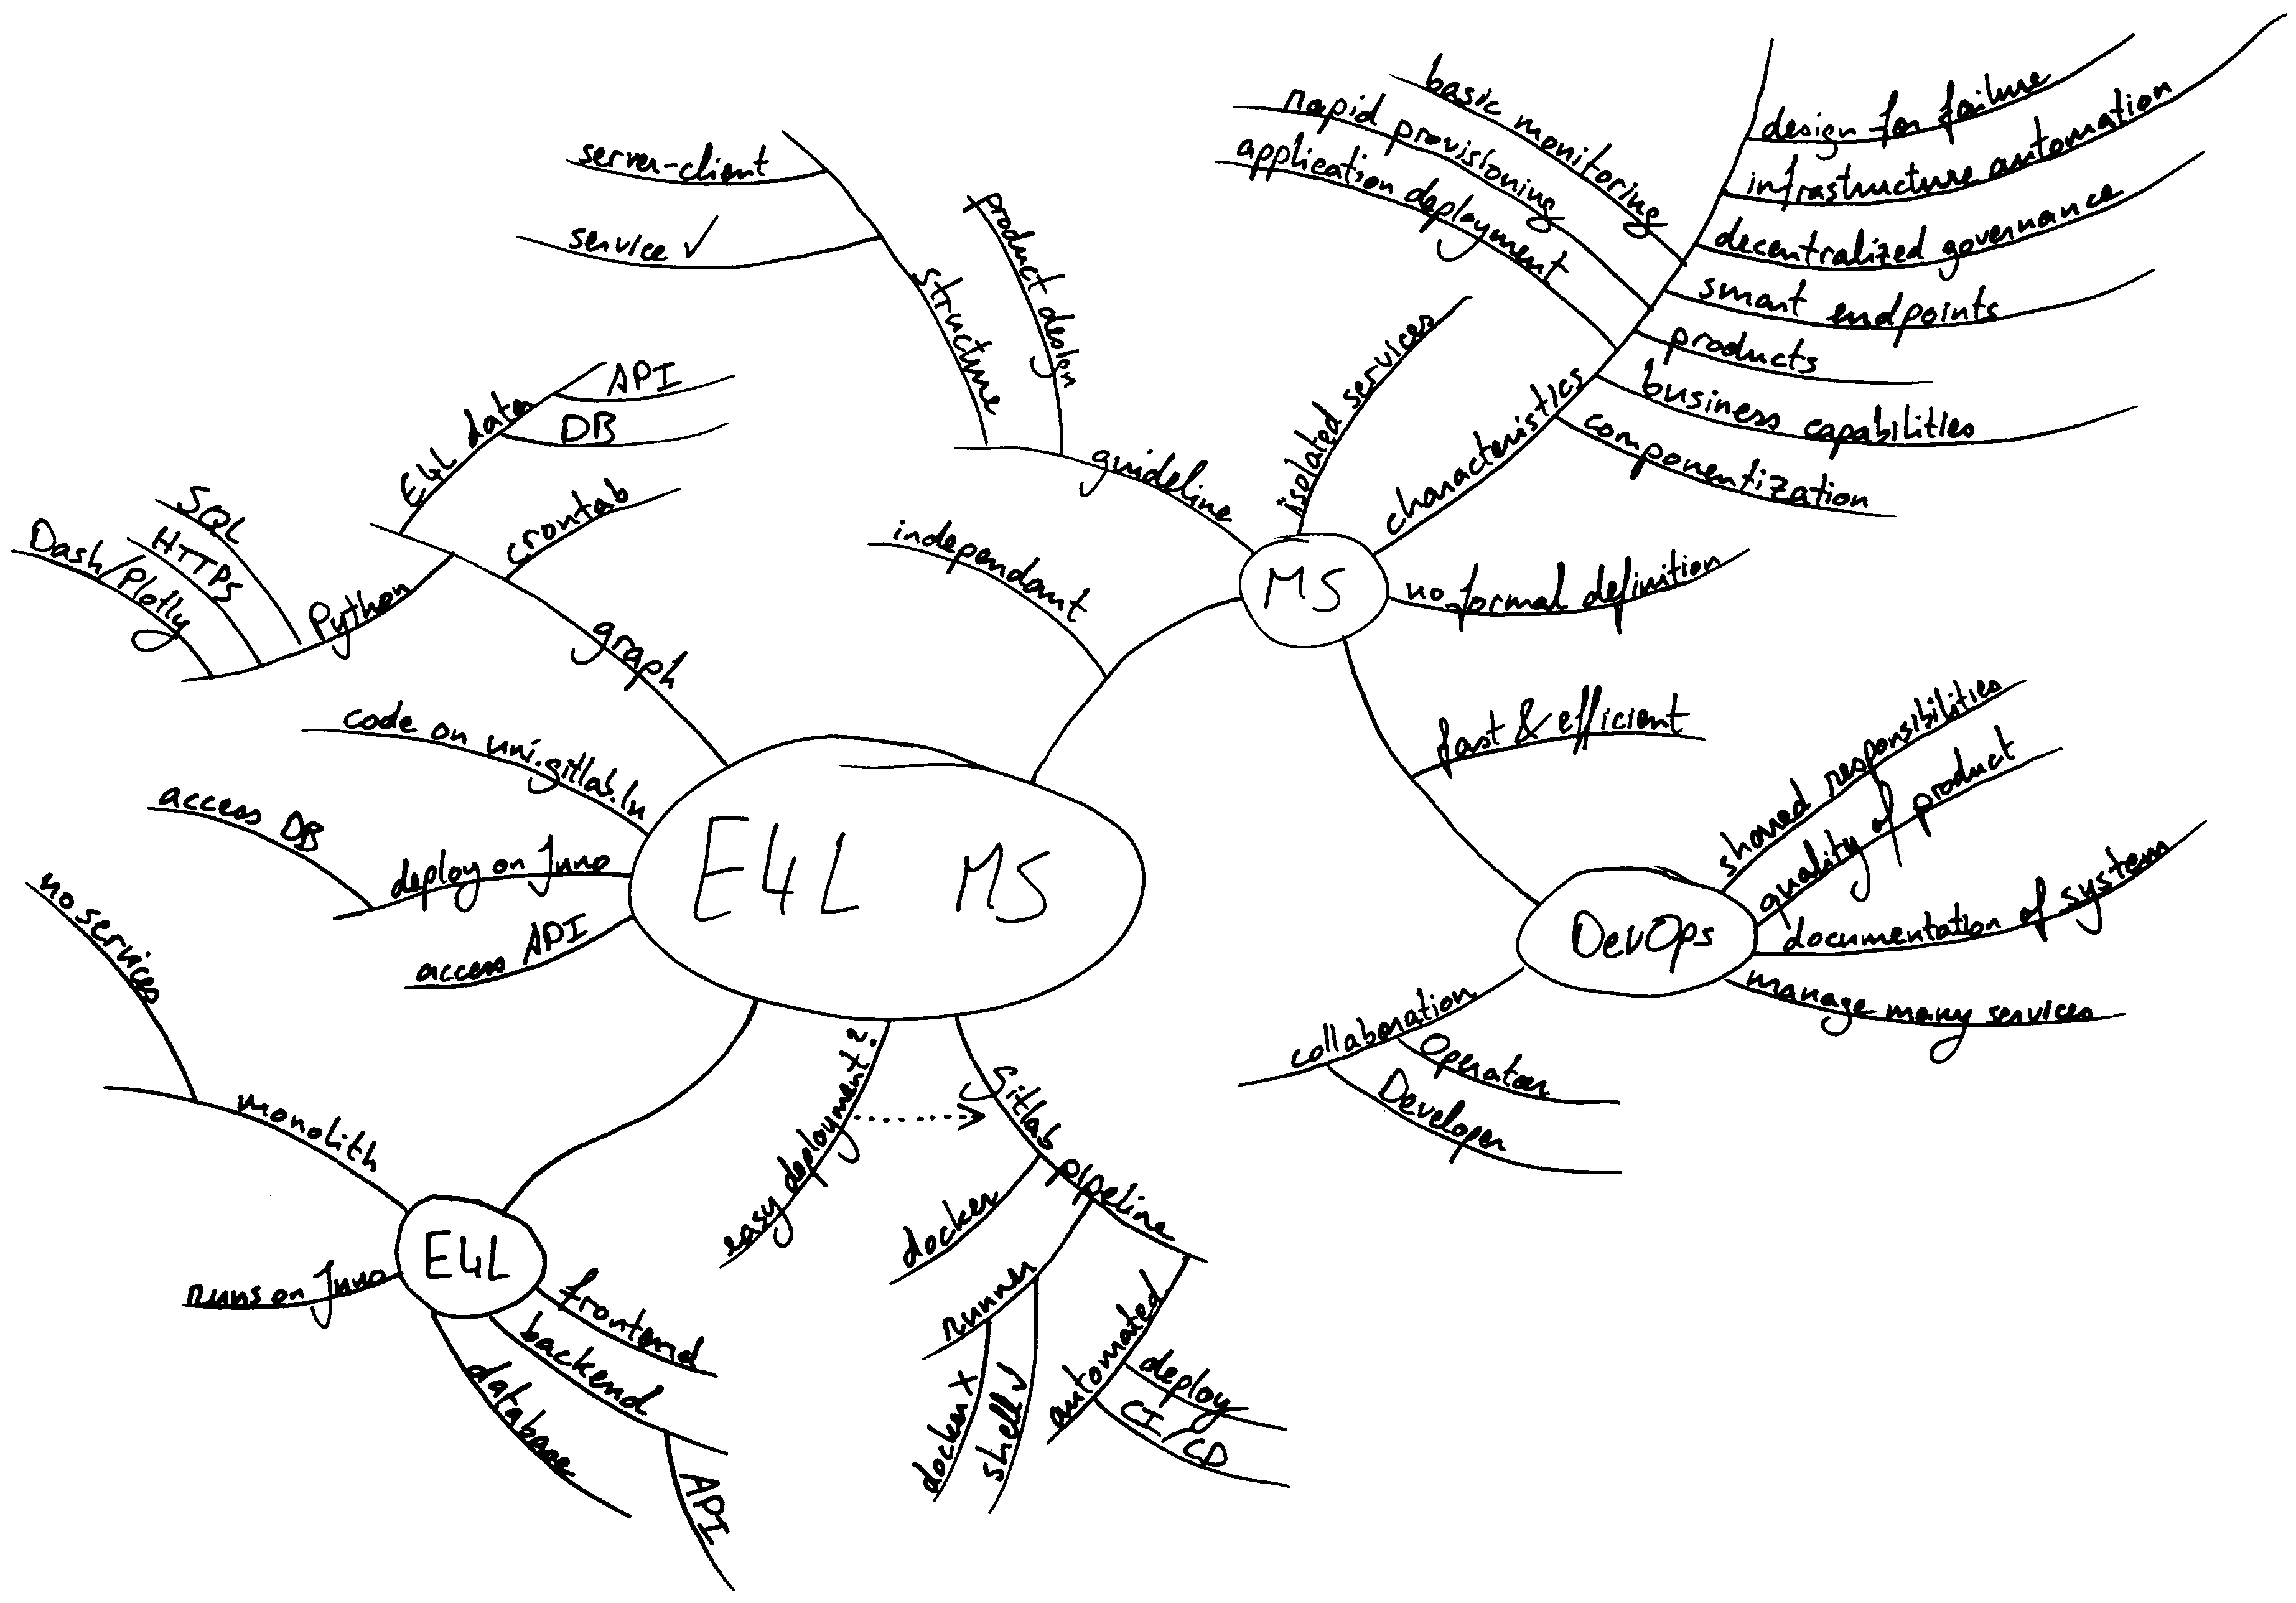
\includegraphics[width=\linewidth]{images/mindmap.png}
	\caption{Mindmap of topics for this BSP}
	\label{fig:mindmap}
\end{figure*}

% \KB{rely on E4L use-case; understand \gls{ms} \& work with GL; etc} 

\subsubsection{Technical deliverables}

The main goal of our technical deliverable was to collect empirical
evidence about how easy it is to deploy a \gls{ms}\footnote{This point
can be found in the bottom branch of the main subject \textit{E4L MS} in Figure
\ref{fig:mindmap}.} given the \gls{e4l} application---which we assume
to be a monolithic application. Given the research presented in
section \ref{sd:ms}, we concluded that a \gls{ms} would not be fitting
the architecture of \gls{e4l}\footnote{Laid out in the \textit{E4L}
node in Figure \ref{fig:mindmap}}. Prior to working on this \gls{bsp}---as
well as was discovered and confirmed during the project while
inspecting the \gls{e4l} code---it was known that this application had
the typical front-end, back-end and database structure. There was also
no notion of services in the \gls{ms}-sense of the word. Hence our
assumption of it being a monolith.

% \KB{MONOLITHIC should be an assumption: list evidence leading to
% assumption + how it affected engineering of MS}.

Due to the fact that \glspl{ms} are supposed to be isolated
components, it was clear from the start that we should not modify the
original \gls{e4l} code for our purposes\footnote{Indicated through
the \textit{independant} branch on the connector between the main subject
and the \textit{MS} subtopic in figure \ref{fig:mindmap}}. In fact, given our use-case
of plotting an arbitrary graph\footnote{Laid out in the branch
\textit{graph} of the main subject in figure \ref{fig:mindmap}} using data provided by \gls{e4l}, our
best bet would be to rely on an API that is exposed or to connect to
its database directly. The worst scenario would be one where neither
were available; in this case we would have no other choice but
to make our own API by modifying the \gls{e4l} code or by creating a
wrapper around other functionality that is exposed by \gls{e4l}.

This technical deliverable will dive into the whole process that we
went through from the beginning until the moment we had the final
\gls{ms} up and running alongside \gls{e4l}. The way we conducted the
experiments was a very iterative process. A little
research on a given matter would help us get familiar with a
particular topic as well as how to approach the implementation. We
would then create a dummy code to test said features and keep it
around as a reference in case something breaks in the main
implementation. From there it was a matter of fixing issues that arose
as well as adapting and refining the solution until we obtained the
product we sought to create. If further features were required, we
introduced them step by step by following this iterative process which
was accompanied by lots of dummy implementations for reference and
testing.

% \KB{define methodology for conducting experiments}

However, before being able to fully realise this task there were some
notions that we needed to acquire and get familiar with. First of all,
what even is a \gls{ms}? Further, given that we were working using
GitLab and wanted to take advantage of its \gls{cicd} framework, we
naturally wanted to find out how the concepts of DevOps and \glspl{ms}
were related---since \gls{cicd} is also employed in the DevOps context.


% {\color{gray}
% Provide a synthetic and abstract description of the technical deliverables that were targeted to be produced. 
% }

\subsubsection{Scientific deliverables}

The first scientific deliverable therefore consists in inspecting what
a \gls{ms}\footnote{See \textit{MS} subtopic in figure
\ref{fig:mindmap}} is. Given how this \gls{bsp} revolves around \glspl{ms},
it was essential to learn about them and what is considered
to be a \gls{ms}. Once we had this notion we could expand on it and
construct a meaningful service for the technical part.

The second deliverable consisted in finding out how DevOps\footnote{See
\textit{DevOps} node in figure \ref{fig:mindmap}} plays a
role in the \gls{ms} philosophy\footnote{This is not explicitly laid out
in figure \ref{fig:mindmap}}. There were quite a few aspects
that hinted at a correlation but we wanted to find out where and how
both interplay. This in turn would directly feed back into the
technical deliverable as we would obtain a better overview on the
overall structure and approach.

The \gls{ms} part was of importance in order to actually create the
service in question, while the DevOps side allowed us to automate
the development process and take care of the many manual steps needed to finally
deploy an application---which would be of great importance if we start
to manage more than one \gls{ms}.

% {\color{gray}
% Provide a synthetic and abstract description of the scientific deliverables that were targeted to be produced. 
% Each BSP must contain some work done according to the principles of the scientific method. It basically means that you should define at least one question related to the knowledge domain of your BSP and follow part of the scientific method process to answer to this question. The description of the work done to answer this question is a scientific deliverable.

% Examples of question could be:
% \begin{itemize}
%   \item Is Python an adequate language for concurrent programs?
%   \item How can we measure the ergonomic of a graphical user interface?
%   \item How can we ensure that a program will not fail?
% \end{itemize}

% An answer to such question should be the result of applying partly or totally the scientific method according to its standard definition which can be found in the literature.

% As you can see in this template, the scientific deliverable is entirely separated from the technical deliverable. Of course it addresses a question more or less closely related to the technical deliverable. 
% }


{\color{gray}
\section{Pre-requisites ([5\%..10\%] of total words)} 
Describe in these sections the main scientific and technical knowledge that is required to be known by you before starting the project.
Do not describe in details this knowledge but only abstractly. All the content of this section shall not used, even partly, in the deliverable sections.

\subsection{Scientific pre-requisites}
\subsection{Technical pre-requisites}
}

% \refstepcounter{sdel}
\section{ A Scientific Deliverable 1}
For each scientific deliverable targeted in section~\ref{sec-deliverables} provide a full section with all the subsections described below.
\label{sec-production}

%\input{contents/scientific-deliverables/SD-<name>.tex}
\subsection{Requirements (± 15\% of section's words)}
Describe here all the properties that characterize the deliverables you produced. It should describe, for each main deliverable, what are the expected functional and non functional properties of the deliverables, who are the actors exploiting the deliverables. It is expected that you have at least one scientific deliverable (e.g. ``Scientific presentation of the Python programming language'', ``State of the art on quality models for human computer interaction'', \ldots.) and one technical deliverable (e.g. ``BSProSoft - A python/django web-site for IT job offers retrieval and analysis'', \ldots). 
\subsection{Design (± 30\% of section's words)}
Provide the necessary and most useful explanations on how those deliverables have been produced.
\subsection{Production (± 40\% of section's words)}
Provide descriptions of the deliverables concrete production. It must present part of the deliverable (e.g. source code extracts, scientific work extracts, \ldots) to illustrate and explain its actual production.
\subsection{Assessment (± 15\% of section's words)}
Provide any objective elements to assess that your deliverables do or do not satisfy the requirements described above. 

\refstepcounter{tdel}
\section{Technical Deliverable \thetdel\ -- Does E4L allow for easy
deployment of adjacent Microservices?}

\subsection{Requirements}

Our case study consisted in creating a \gls{ms} relying on the
\gls{e4l} application. The latter is built using a monolithic
architecture, and we want to find out how easy it is to deploy an
adjacent \gls{ms} application.

The \gls{ms} to be created should allow us to test the hypothesis that
\glspl{ms} are easy to create and deploy. Further, it should fit into
our \gls{e4l} case study---we will have our service display a graph
based on data collected by the \gls{e4l} application.  To close
everything off, we shall also create a GitLab pipeline that automates
the deployment of this \gls{ms}.

Hence, the design section will tackle all the steps we had to
undertake in order to reach the final and fully automated deployment
pipeline. The production section will dive into the technical details
and difficulties of each step. The assessment is going to lay out our
judgement on how easy it was to deploy the \gls{ms} given the current
\gls{e4l} application architecture.

\subsection{Design}

\KB{Methodlogy: Steps required to achieve final solution}

\subsection{Production}

\KB{More details on each step + difficulties encountered}

\subsection{Assessment}

\KB{Was is easy to deploy \gls{ms}?}


% {\color{gray}
\section*{Acknowledgment}

I would like to thank my tutor Alfredo Capozucca for being very
pleasant to work with. He would always take his time to explain or
clarify some things and made sure I understood what is going on. In
addition, when in doubt or stuck he was happy to help and always gave
me the right hints and nudges to the correct path.

In addition, I also want to thank Boris Floka who is a prior team
member of E4L and had great responsibility in creating the back-end.
Figuring out how to properly obtain data from \gls{e4l} was not very
obvious and he was very responsive and happy to help me achieve this.

% The authors would like to thank the BiCS management and education team for the amazing work done.
% }

% {\color{gray}
\section{Conclusion}

Creating this \gls{ms} was quite a challenge, mainly due to the many
unforeseen issues with the various tools. It is hard to say if a lot
of these issues could have been avoided by simply using a different
programming language than Python. Given how the original \gls{e4l}
code was written in Java and did not seem to have faced similar
problems, there is reason to suspect the Python libraries we used had
some trouble coping with our setting.

Overlooking the numerous roadblocks, the process of creating the
\gls{ms} was rather straightforward. This was further boosted by the
clear boundaries between the monolith and the service, which avoided
us from having to dive into the \gls{e4l} code in order to integrate
our functionality. Thus, a key to success is the clear definition and
specification of service interfaces. We were therefore able to implement our service
without too much regard to the original code base. The end result of
having an automated pipeline further eases the development greatly---now
modifications will automatically be deployed without manual
intervention.

One should note however, that we worked in a very simplified and
almost \emph{sandbox-like} setting with only a single \gls{ms} coupled to
a monolith. We did not have to worry about managing multiple
\glspl{ms} and deal with all the complexities that stem from this. It
would therefore be interesting to further investigate how \glspl{ms} would
behave in a more real setting where a lot of interplay between a
greater network of services and teams needs to be taken care of.

% The conclusion goes here.
% }


% An example of a floating figure using the graphicx package.
% Note that \label must occur AFTER (or within) \caption.
% For figures, \caption should occur after the \includegraphics.
% Note that IEEEtran v1.7 and later has special internal code that
% is designed to preserve the operation of \label within \caption
% even when the captionsoff option is in effect. However, because
% of issues like this, it may be the safest practice to put all your
% \label just after \caption rather than within \caption{}.
%
% Reminder: the "draftcls" or "draftclsnofoot", not "draft", class
% option should be used if it is desired that the figures are to be
% displayed while in draft mode.
%
%\begin{figure}[!t]
%\centering
%\includegraphics[width=2.5in]{myfigure}
% where an .eps filename suffix will be assumed under latex, 
% and a .pdf suffix will be assumed for pdflatex; or what has been declared
% via \DeclareGraphicsExtensions.
%\caption{Simulation results for the network.}
%\label{fig_sim}
%\end{figure}

% Note that the IEEE typically puts floats only at the top, even when this
% results in a large percentage of a column being occupied by floats.


% An example of a double column floating figure using two subfigures.
% (The subfig.sty package must be loaded for this to work.)
% The subfigure \label commands are set within each subfloat command,
% and the \label for the overall figure must come after \caption.
% \hfil is used as a separator to get equal spacing.
% Watch out that the combined width of all the subfigures on a 
% line do not exceed the text width or a line break will occur.
%
%\begin{figure*}[!t]
%\centering
%\subfloat[Case I]{\includegraphics[width=2.5in]{box}%
%\label{fig_first_case}}
%\hfil
%\subfloat[Case II]{\includegraphics[width=2.5in]{box}%
%\label{fig_second_case}}
%\caption{Simulation results for the network.}
%\label{fig_sim}
%\end{figure*}
%
% Note that often IEEE papers with subfigures do not employ subfigure
% captions (using the optional argument to \subfloat[]), but instead will
% reference/describe all of them (a), (b), etc., within the main caption.
% Be aware that for subfig.sty to generate the (a), (b), etc., subfigure
% labels, the optional argument to \subfloat must be present. If a
% subcaption is not desired, just leave its contents blank,
% e.g., \subfloat[].


% An example of a floating table. Note that, for IEEE style tables, the
% \caption command should come BEFORE the table and, given that table
% captions serve much like titles, are usually capitalized except for words
% such as a, an, and, as, at, but, by, for, in, nor, of, on, or, the, to
% and up, which are usually not capitalized unless they are the first or
% last word of the caption. Table text will default to \footnotesize as
% the IEEE normally uses this smaller font for tables.
% The \label must come after \caption as always.
%
%\begin{table}[!t]
%% increase table row spacing, adjust to taste
%\renewcommand{\arraystretch}{1.3}
% if using array.sty, it might be a good idea to tweak the value of
% \extrarowheight as needed to properly center the text within the cells
%\caption{An Example of a Table}
%\label{table_example}
%\centering
%% Some packages, such as MDW tools, offer better commands for making tables
%% than the plain LaTeX2e tabular which is used here.
%\begin{tabular}{|c||c|}
%\hline
%One & Two\\
%\hline
%Three & Four\\
%\hline
%\end{tabular}
%\end{table}


% Note that the IEEE does not put floats in the very first column
% - or typically anywhere on the first page for that matter. Also,
% in-text middle ("here") positioning is typically not used, but it
% is allowed and encouraged for Computer Society conferences (but
% not Computer Society journals). Most IEEE journals/conferences use
% top floats exclusively. 
% Note that, LaTeX2e, unlike IEEE journals/conferences, places
% footnotes above bottom floats. This can be corrected via the
% \fnbelowfloat command of the stfloats package.

% trigger a \newpage just before the given reference
% number - used to balance the columns on the last page
% adjust value as needed - may need to be readjusted if
% the document is modified later
%\IEEEtriggeratref{8}
% The "triggered" command can be changed if desired:
%\IEEEtriggercmd{\enlargethispage{-5in}}

% references section

% can use a bibliography generated by BibTeX as a .bbl file
% BibTeX documentation can be easily obtained at:
% http://mirror.ctan.org/biblio/bibtex/contrib/doc/
% The IEEEtran BibTeX style support page is at:
% http://www.michaelshell.org/tex/ieeetran/bibtex/
%\bibliographystyle{IEEEtran}
% argument is your BibTeX string definitions and bibliography database(s)
%\bibliography{IEEEabrv,../bib/paper}
%
% <OR> manually copy in the resultant .bbl file
% set second argument of \begin to the number of references
% (used to reserve space for the reference number labels box)
\begin{thebibliography}{1}
	% vim: nowrap fdm=marker foldlevel=0 tw=0
% {{{
{\color{gray}
\bibitem[BiCS(2018a)]{bics-bsp-report-template}
\newblock {BiCS Bachelor Semester Project Report Template.}
\newblock \url{https://github.com/nicolasguelfi/lu.uni.course.bics.global}
\newblock {University of Luxembourg, BiCS - Bachelor in Computer Science (2017).}

\bibitem[BiCS(2018b)] {bics-bsp-reference-document}
\newblock {Bachelor in Computer Science}:
\newblock {BiCS Semester Projects Reference Document}.
\newblock Technical report, University of Luxembourg (2018)

\bibitem[Armstrong and Green(2017)]{armstrong2017guidelinesforscience}
\newblock J~Scott Armstrong and Kesten~C Green.
\newblock Guidelines for science: Evidence and checklists.
\newblock \emph{Scholarly Commons}, pages 1--24, 2017.
\newblock \url{https://repository.upenn.edu/marketing\_papers/181/}
}
% }}}


\bibitem{ms-definition}
\newblock{Microservices: A definition of this new architectural term}
\newblock{\url{https://martinfowler.com/articles/microservices.html}}

\bibitem{central-decentral}
\newblock{Centralized and Decentralized Management Explained}
\newblock{\url{https://content.personalfinancelab.com/finance-knowledge/management/centralized-and-decentralized-management-explained/?v=c4782f5abe5c}}

\bibitem{ms-trade-off}
\newblock{Microservice Trade-Offs -- Operational Complexity (Con)}
\newblock{\url{https://martinfowler.com/articles/microservice-trade-offs.html\#ops}}

\bibitem{pipelines}
\newblock{DeploymentPipeline}
\newblock{\url{https://martinfowler.com/bliki/DeploymentPipeline.html}}

\bibitem{devops-culture}
\newblock{DevOpsCulture}
\newblock{\url{https://martinfowler.com/bliki/DevOpsCulture.html}}

\bibitem{ms-prereq}
\newblock{MicroservicePrerequisites}
\newblock{\url{https://martinfowler.com/bliki/MicroservicePrerequisites.html}}

\bibitem{sos-survey}
\newblock{A Survey on the Interplay between Software Engineering and Systems Engineering during SoS Architecting}
\newblock{Héctor Cadavid, Vasilios Andrikopoulos, Paris Avgeriou, John Klein}

\bibitem{docker-so}
\newblock{Challenges in Docker Development: A Large-scale Study Using Stack Overflow}
\newblock{Mubin Ul Haque, Leonardo Horn Iwaya, M. Ali Babar}

\bibitem{ms-arch-study}
\newblock{Architecting with microservices: A systematic mapping study}
\newblock{Paolo Di Francesco, Patricia Lago, Ivano Malavolta}

\bibitem{ms-challenges}
\newblock{Challenges of production microservices}
\newblock{Benjamin Götz, Daniel Schel, Dennis Bauer, Christian Henkel, Peter Einberger, Thomas Bauernhansl}

\bibitem{ms-pains-gains}
\newblock{The pains and gains of microservices: A Systematic grey literature review}
\newblock{Jacopo Soldani, Damian Andrew Tamburri, Willem-Jan Van Den Heuvel}

\bibitem{}
\newblock{}
\newblock{\url{}}

\end{thebibliography}
\newpage 
\section{Appendix}
{\color{gray}
All images and additional material go there.
}

\subsection{Benefits of microservices}
\label{app:ms-benefit}

To understand the benefits and motivations behind using \gls{ms} over
the monolithic style, we will first look at the latter.
\cite{ms-definition}

Monolithic architectures build applications using a single unit. This
basically means that all of an application's functionality, logic,
classes, function and name spaces are in the end located within a
single executable and thus run within a single process.
\cite{ms-definition} This model is very much usable in fact and allows
us to create functioning systems---as has demonstrated the time of
software development before \glspl{ms} were introduced. However, this
architectural style raises some issues nonetheless. For instance, even
the smallest of changes in an application require the whole product to
be rebuilt and redeployed or redistributed which is not necessarily
ideal in the case of large applications with multiple end-users.

As the application's life cycles goes on, it is unavoidable to modify
it over time. In a monolithic system however, it becomes increasingly
difficult to maintain a modular structure---if one was present to
begin with---which in turn also leads to modifications becoming more
expensive. \cite{ms-definition} The expensive modifications are
explained by the fact that if a modular structure cannot be
guaranteed, it possibly entails that changes to one component may
impact other components which were not supposed to be affected.
\cite{ms-definition} This may result in many adjacent changes and
unexpected issues to be performed and treated respectively.

Lastly, if we want to scale an application we actually need to scale
the application as a whole rather than the individual components that
need to be scaled.

\begin{figure*}
	\centering
	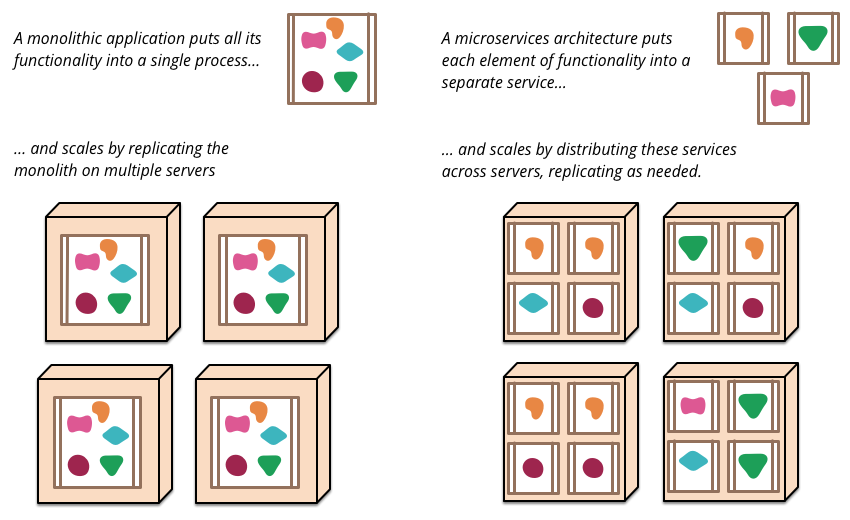
\includegraphics[width=0.75\linewidth]{images/sketch.png}
	\caption{Monoliths and Microservices \cite{ms-definition}}
	\label{fig:monoliths-ms}
\end{figure*}

Figure \ref{fig:monoliths-ms} nicely demonstrates some of the
aforementioned issues and how the \gls{ms} architecture tries to
tackle them.

Since the application is now split into separate services, making
modifications will not require us to build and deploy the whole
application anew. It will be enough to only update the services in
question.

Further, the fact that the application is built in a modular fashion
from the ground up and divided into smaller chunks and services makes
it easier to maintain a modular structure within the application as a
whole. As a result, making changes to one such service will guarantee
that none of the other services will be affected and thus keep
undesired or unforeseen side effects to a minimum.

We can also see that scaling an application becomes much less of a
burden. No longer do we need to scale the whole application, but we
can simply introduce new services where needed.


\subsection{Obtaining data from E4L}
\label{app:e4l-data}

To give an outline, our first attempt was to sort of brute-force our
way into obtaining data. While not the most useful of data, it was
something to work with. Only later have we discovered that \gls{e4l}
exposes an API which greatly alleviates the burden of our brute-force
approach.

Obtaining useful data however, was only achievable thanks to the help
and guidance of a prior team member of \gls{e4l} who had great
responsibility in creating the back-end. He showed me the proper way to
obtain all the data from the API as well as by directly connecting to
the \gls{e4l} database.

\paragraph{First attempt at obtaining data from the back-end}

Upon inspection of the \gls{e4l} backend, we were able to find a
potentially relevant endpoint that would allow us to query answers
from the questionnaire.  However, it quickly became apparent that the
back-end endpoints were specifically made to be used by the front-end
page. Further evidence for this can be found in the functionalities
described in the README, which also informs us that the only data that
can be extracted is specific to a session. All of this essentially
means that we have no direct way to access any data beyond what we are
presented with on the web page---which would only comprise our results
from after answering the questionnaire.

Upon completing the questionnaire in E4L, we are presented the
following page\footnote{Note that the ID will be different. This is an
example for a results page that we obtained at some point.}:
\url{https://juno.uni.lux/e4l/result/MzA5.-7-sMYXmv3tXyuLQT2s1ZgULRKY}.
The so-called	\textit{sessionId} is unique to our provided answers, so
by taking note of it we are able to review our \textit{energy scores}
at any point in time. The obvious course of action now would be to use
the \verb|/calculate/session/{sessionId}| endpoint---which is our only
of two GET handlers regarding the questionnaire---to obtain our
results.

One problem rose quickly however: We had no information on where or
how to access the back-end in order to issue our GET request. Upon
inspection in the code for both the front-end and back-end, we were
unable to find any concrete traces on how to reach it. The closest we
managed to find was the definition of a \verb|baseUrl| using \verb|axios|,
but that still left us clueless. So we set out to create a web scraper
that would parse the HTML of the above results page.

\paragraph{Scraping the results page for data}

We used \verb|selenium| to perform this task. However, running the
selenium browser in headless mode---as is required for running this
code in a docker container---caused issues with our scraper. It turns
out that the page contents would not be loaded unless the page was
actually rendered by the browser. In addition to this approach being
extremely slow due to \verb|selenium|, it was simply not usable for
our use-case.

\paragraph{Obtaining data from the back-end API}

It was only after a third and final inspection of the E4L
code---performed while documenting what we did---with the help of
GitLab's search utility, that we discovered how to access the
back-end.  It was hidden in plain site in the front-end README,
however it was not emphasised very well which caused us to completely
overlook it at multiple occasions.

That said, we were able to retrieve our results using the API by
issuing a GET request on
\\\url{https://juno.uni.lux/e4lapi/calculate/session/MzA5.-7-sMYXmv3tXyuLQT2s1ZgULRKY}.
However, some data about global statistics (i.e. Luxembourg, Europe,
World) were not available as they seemed to be hard coded into the
front-end.

\paragraph{Obtaining all the data by querying the API and database}

This step is elaborated on in the technical production section
\ref{sec:e4l-data-query}

% that's all folks
\end{document}


